\documentclass[12pt]{article}
\usepackage[latin1]{inputenc}
\usepackage[T1]{fontenc}
\usepackage{amsmath}
\usepackage{amsfonts}
\usepackage{graphicx}
\usepackage{float}
\usepackage{amssymb}
\usepackage{makeidx}
\usepackage{multicol}
\usepackage{fancyhdr}
\usepackage{setspace}
\usepackage{graphicx}
%\usepackage{showframe}
\usepackage{geometry}
\geometry
	{letterpaper,
	textwidth=17.6cm,
	top=2.5cm,
	head=1cm,
	headsep=2mm}
\pagestyle{fancy}
\fancyhead[R]{\thepage}
\setlength{\parskip}{0.7cm}
\setlength{\parindent}{0.5cm}
\cfoot{}



	\title{Hints   on   halo   evolution   in   SFDM  models   with   galaxy  observations}
	\author{
		Alma  X.  Gonz�lez-Morales$^{1}$, Alberto  Diez-Tejedor$^{2}$,\\ L.  Arturo  Ure�a-L�pez$^{2}$, and  Octavio  Valenzuela$^3$\\ \\
		$^{1}${\small Instituto de Ciencias Nucleares, Universidad Nacional Aut�noma de M�xico,}\\ {\small Circuito   Exterior   C.U.,    A.P.   70-543,    M�xico   D.F.   04510,    M�xico.}\\  $^{2}${\small Departamento   de   F�sica,    Divisi�n   de   Ciencias   e   Ingenier�as,}\\
		{\small Campus   Le�n,    Universidad   de   Guanajuato,    Le�n   37150,    M�xico}\\
		$^{3}${\small Instituto de Astronom�a, Universidad Nacional Aut�noma de M�xico,}\\ {\small Circuito   Exterior   C.U.,    A.P.   70-264,    M�xico   D.F.   04510,    M�xico.}}	

\begin{document}
	\maketitle
	A massive, self-interacting scalar field has been considered as a possible candidate for the dark matter in the universe. We present an observational constraint to the model arising from strong lending observations in galaxies. The result points to a discrepancy in the properties of scalar field dark matter halos for dwarf and lens galaxies, mainly because halo parameters are directly related to physical quantities in the model. This is an important indication that it becomes necessary to have a better understanding of halo evolution in scalar field dark matter models, where the presence of baryons can play an important role.\\
		
	\begin{multicols*}{2}
		
		\begin{center}
			\section{INTRODUCTION}
		\end{center}
		
		\small
		The nature of dark matter (DM) remains elusive today, even though a generic cold particle weakly coupled to the standard model seems to be the most promising candidate.\cite{bruegmann_binary_1999} Treating DM as a bunch of classical particles is an appropriate efective description for many physical situations. However, if DM is composed of bosons, the zero mode can develop a non-vanishing expectation value; this efect is usually known as Bose-Einstein condensation. A condensed phase does not admit a description in terms of classical particles, and the concept of a coherent excitation (i.e. a classical feld) is more appropriate for practical purposes \cite{sikivie_bose-einstein_2009}. A species realization of this scenario can be provided by the axion \cite{robles_flat_2012}, see also \cite{bernal_flat_nodate}. 
		
		In this paper we shall explore the lensing properties of a generic model of DM particles in a condensate, and compare the conditions necessary to produce strong lensing with those required to explain the dynamics of dwarf galaxies. As a result we will get some insight into halo evolution arising from this type of models. 
		
		In particular, we will consider the case of a complex, massive, self-interacting scalar feld $\phi$ satisfying the Klein-Gordon (KG) equation, $\phi=-(mc/\hbar)^2\phi-\gamma (\|\phi|)^2 \phi =0$, with the box denoting the d?Alembertian operator in four dimensions. For those natural situations in which the scalar ?eld mass $m$ is much smaller than the Planck scale, $m_{Plank} = (\hbar c/G)^{1/2}$, such that $\Lambda \equiv \gamma m^{2}_{Planck}/4\pi m^2 \gg 1 $ the coherent (self-gravitating, spherically symmetric) solutions to the KG equation ad- mit a very simple expression for the mass density \cite{lee_galactic_1996} \cite{arbey_galactic_2003}.
		
		\begin{eqnarray}\rho (r) = \{ \rho {\sin(\pi r /r_{max})/(\pi r/r_{max})}
		\label{ECUACION 1}
		\end{eqnarray}
	 
		As usual we will refer to this model as scalar ?eld dark matter (SFDM). Here $r_{max} \equiv \sqrt{\pi^2 \Lambda /2} (\hbar / mc)$ is a constant with dimensions of length (notice that $r_{max}$ is just the Compton wavelength of the scalar particle, $\hbar /mc$, scaled by a factor of order $\Lambda^{1/2}$ ), and $\rho_c$ the density at the center of the configuration. The mass density pro?le in Equation \ref{ECUACION 1} leads to compact objects of size $r_{max}$ , and typical masses, $4\rho_c r^3_{max} /\pi$, that vary from configuration to configuration   according   to   the   value   of   the   central   density.
		
		Equation \ref{ECUACION 1} was obtained without taking into account the gravitational influence of any other matter sources, and assuming that all the scalar particles are in the condensate. It has been used as a first order approximation to describe the distribution of matter in dwarf spheroidal, which are expected to be DM dominated. The mass distribution would be smooth close to the center of these galaxies, alleviating the cusp/core problem motivated by the discrepancies between the observed high resolution rotation curves and the profiles suggested by N-body simulations \cite{de_blok_h_2002}; see however \cite{gonzalez-morales_hints_2013}.
		
		The      dynamics      of      dwarf      galaxies      suggests      a      self interacting   scalar   with   $m^4 / \gamma \sim 50-75(eV/c^2)^4$,    (i.e. $r_{max} \sim 5.5-7Kcp$), and typical central densities of the order of $\rho_c \sim 10^{-3} M/pc^3$, see \cite{bernal_flat_nodate}. We are aware that Milky Way size galaxies are, at least, an order of magnitude larger than this value of $r_{max}$ , and then they do not ?t in this model as it stands. Nonetheless, if not all the DM particles are in the condensate, there is a possibility to have gravitational configurations where the inner regions are still described by the mass density pro?le in Equation \ref{ECUACION 1}, wrapped in a cloud of non-condensed particles \cite{valenzuela_is_2007}. For the purpose of this paper we do not need to specify the complete halo model. This is because strong lensing is not very sensitive to the mass distribution outside the Einstein radius, at most of the order of a few Kpc, just bellow the expected value of $r_{max}$ . We could not neglect the exterior pro?le of the halo if we were interested,  for  instance,  in  weak  lensing  observations.
		
		\section{LENSING PROPERTIES OF SFDM HALOS}
		
		In the weak field limit the gravitational lensing produced by a mass distribution can be read directly from the density pro?le. As usual we assume spherical symmetry, and use the thin lens approximation, that is, the size of the object is negligible when compared to the other length scales in the con?guration, i.e. the (angular) distances between the observer and the lens, $D_{OL}$, the lens and the source, $D_{LS}$, and from the observer to the source, $D_{OS}$.
		
		Under   these   assumptions   the   lens   equation   takes   the form
		\begin{eqnarray}
			\beta = \theta -\frac{M(\theta)}{\pi D^2_{OL}\theta \Sigma_{cr}}
			\label{ECUACION 2}
		\end{eqnarray}
		with $\beta$ and $\theta$  denoting the actual (unobservable) angular position of the source, and the apparent (observable) angular position of the image, respectively, both measured with respect to the line-of-sight \cite{bertone_particle_2005}. The (projected) mass enclosed in a circle of radius $\xi$, $M(\xi)$, is de?ned from the (projected) surface mass density, $\Sigma (\xi)$ throug
		\begin{eqnarray}
		\Sigma(\xi) \equiv \int_{-\infty}^{\infty}dz \rho (z,\xi),	M(\xi) \equiv 2\pi \int_{0}^{\xi} d\xi' \xi' \Sigma (\xi'). 
		\label{ECUACION 3}
		\end{eqnarray}
	
		Here $\xi = D_{OL} \theta$ is a radial coordinate in the lens plane, and z a coordinate in the orthogonal direction. Finally $\Sigma_{cr} \equiv c^2 D_{OS} /4\pi GD_{OL} D_{LS}$ is  a  critical  value  for  the  surface density.
		
		In general, Equation \ref{ECUACION 2} will be non-linear in $\theta$, and it could be possible that for a given position of the source, $\beta$, there would be multiple solutions (i.e. multiple images) for the angle $\theta$. This is what happens in the strong lensing regime to be discussed below. One particular case is that with a perfect alignment between the source and the lens, that actually de?nes the Einstein ring, with an angular radius of $\theta_E \equiv \theta (\beta = 0)$.
		
		For    a    SFDM    halo,    and    in    terms    of    the    normalized lengths   $\xi_* \equiv \xi /r_{max}$    and   $z_* \equiv z/r_{max}$,   the   surface   mass density  takes  the  form
		{\small 
		\begin{eqnarray}
			\Sigma_{SFDM}(\xi_*)= \dfrac{2\rho_c r_{max}}{\pi}\int_{0}^{z_{max}}\frac{\sin(\pi\sqrt{\xi^2_* +z^2_*})}{\sqrt{\xi^2_*+z^2_*}} dz_*
			\label{ECUACION 4}
		\end{eqnarray}}
		with $0\leq \xi?* \leq 1$ and $z_{max} =\sqrt{1-\xi^2_*}$. A similar expression can be obtained for the mass enclosed in a circle or radius $\xi$, see Equation \ref{ECUACION 3} above. Here we are not considering the e?ect of a scalar cloud surrounding the condensate. For $r \lesssim r_{max}$ this will appear as a projection effect, which is usually considered to be small \cite{boehm_scalar_2004}. Indeed, we have corroborated that the inclusion of an outer isotherm sphere does not affect the conclusions of this paper.
		
		With  the  use  of  the  expression  for  the  projected  mass, $M_{SFDM}(\xi_*)$,  the  lens  equation  simplifies to
		\begin{eqnarray}
			\beta_* (\theta_*)=\theta_* -\bar{\lambda}\frac{m(\theta_*)}{\theta_*},
			\label{ECUACION 5}
		\end{eqnarray}
		\begin{figure}[H]
			\centering
		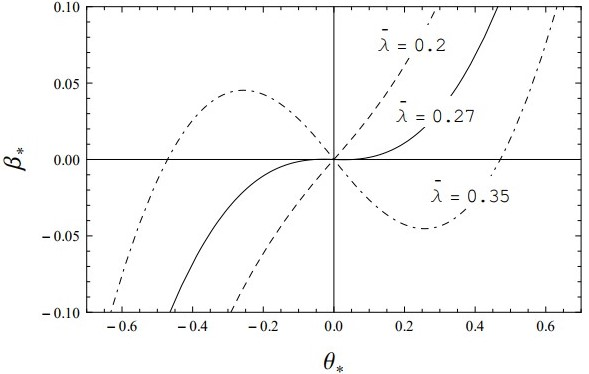
\includegraphics[width=8cm]{GRAFICO 1}
		\caption{The lens equation of a SFDM halo model, Equation \ref{ECUACION 5}, as a function of $\bar{\lambda}$. The roots de?ne the Einstein radius, $\theta_{*E}$, and its local maximum (minimum) the critical impact parameter, $\beta_{*cr}$. Both quantities are well de?ned only for values of $\bar{\lambda} > \bar{\lambda}_{cr} \simeq 0.27$, which  is  the  threshold  value  for  strong  lensing.}
		\label{GRAFICO 1}
		\end{figure}
		where $m(\xi_*) \equiv M_{SFDM}(\xi_*)/\rho_c r^3_{max}$ is a normalized mass function, evaluated numerically. Here $\beta_* = D_{OL}\beta /r{max}$ and $\theta_* = D_{OL} \theta / r_{max}$ are the normalized angular positions  of  the  source  and  images,  respectively,  and  the  parameter $\bar{\lambda}$  is  given  by
		\begin{eqnarray}
			\bar{\lambda} \equiv \frac{\rho_c r_{max}}{\pi \Sigma_{cr}} = 0.57h^{-1} (\frac{\rho_c}{M pc^{-3}})(\frac{r_{max}}{kpc})\frac{d_{OL}d_{LS}}{d_{OS}}
			\label{ECUACION 6}
		\end{eqnarray}		
		
		In order to avoid confusion with the self-interaction term, $\lambda$, we have introduced a bar in the new parameter $\bar{\lambda}$. We have also de?ned the reduced angular distances $d_A\equiv D_AH_0/c$, and considered $H_0 \equiv 100h(km/s)/Mpc$ as the Hubble  constant  today,  with  $h=0.710 \pm 0.025$  \cite{jarosik_seven-year_2011}.
		
		In  Figure \ref{GRAFICO 1}  we  show  the  behavior  of  the  lens  Equation \ref{ECUACION 5} as the $\bar{\lambda}$ parameter varies (i.e. for di?erent values of the combination $\rho_c r_{max}$ ). Some notes are in turn: i) Strong lensing can be produced only for configurations with $\bar{\lambda} > \bar{\lambda}_{cr} \simeq 0.27$, and   ii)   For   these configurations,   only   those with an impact parameter $|{\beta_*}| < \beta_{*cr}$ can produce three images (note that the actual value of ??cr depends on the parameter $\bar{\lambda}$, $\beta_{*cr}(\bar{\lambda})$).
		
		These conditions on the SFDM pro?le are very similar to those obtained for the Burkert model in \cite{bruegmann_binary_1999}; this is not surprising because both of them have a core in radius. In that sense SFDM halos are analogous to those proposed by Burkert \cite{sikivie_bose-einstein_2009}, but with the advantage that their prop- erties are clearly connected to physical parameters in the model.
		
		In   Figure \ref{GRAFICO 2}   we   show   the   magnitude   of   the   Einstein   ra- dius,  $\theta_{*E}$ ,   as   a   function   of   the   parameter   $\bar{\lambda}$,   where   for comparison we have also plotted the same quantity for the NFW \cite{robles_flat_2012} and Burkert \cite{bruegmann_binary_1999} pro?les. The minimum value of $\bar{\lambda}$ needed to produce multiple images is higher for a  SFDM  halo, $\bar{\lambda}^{NFW}_{cr} = 0 < \bar{\lambda}^{Burkert}_{cr} = 2/\pi^2 < \bar{\lambda}^{SFDM}_{cr} \simeq 0.27$. (Notice that there is an extra factor of $1/4\pi$ in our definition of $\bar{\lambda}$ when compared to that reported in \cite{bruegmann_binary_1999}.) SFDM halos seem to require larger values of
		\begin{figure}[H]
			\centering
		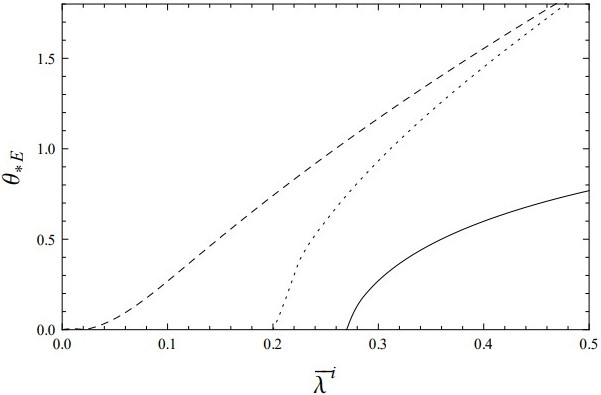
\includegraphics[width=8cm]{GRAFICO 2}
		\caption{The Einstein radius, $\theta_{*E}$, as function of $\bar{\lambda}^i$, for SFDM (solid line), NFW (dashed line), and Burkert (dotted
		line) halo models. Einstein rings of similar magnitude require $\bar{\lambda}^{NFW} < \bar{\lambda}^{Burkert} < \bar{\lambda}^{SFDM}$}.
		\label{GRAFICO 2}
		\end{figure}
		$\bar{\lambda}$ in order to produce Einstein rings of similar magnitude to those obtained for the other pro?les, but this is in part due to projection e?ects that have not been considered in this paper \cite{boehm_scalar_2004} \cite{bernal_flat_nodate}.
		
		\section{LENSING   VS   DYNAMICS}
		
		Taking   into   account   that   in   SFDM   models   there   is   a critical   value   for   the   parameter,   $\bar{\lambda}_{cr} \simeq 0.27$,   and   con- sidering  the  definition  in  Equation \ref{ECUACION 6},  we  can  write  the  con- dition  to  produce  strong  lensing  in  the  form
		\begin{eqnarray}
			\rho_c r_{max} [M_\odot pc^{-2}]  \gtrsim 473.68hf_{dist},
			\label{ECUACION 7} 
		\end{eqnarray}
	
		In order to evaluate the right-hand-side (r.h.s.) of Equation \ref{ECUACION 7}, we consider two surveys of multiply-imaged sys- tems, the CASTLES \cite{lee_galactic_1996} and the SLACS \cite{arbey_galactic_2003}. From them we select only those elements for which the red- shifts of the source and the lens have been determined (which amounts to approximately 60 elements in each survey), and calculate the corresponding distance fac- tor fdist for every element in the reduced sample. In CASTLES (SLACS) the distance factors are in the interval $4 \lesssim f_{dist} \lesssim 27$, ($6 \lesssim f_{dist} \lesssim 25$) with a mean value of, and then the r.h.s. of Equation \ref{ECUACION 7} takes on values in the range $1400 - 9000$, $(2000 - 8500)$. Some representative elements from SLACS are shown in Table \ref{TABLA 1} (galaxy lensing). In terms of the mean values, the inequality in Equation \ref{ECUACION 7} translates into
		\begin{eqnarray}
			\rho_c r_{max} [M_\odot pc^{-2}] \gtrsim 2000, (CASTLES)
			\label{ECUACION 8}
		\end{eqnarray}
		\begin{eqnarray}
		\rho_c r_{max} [M_\odot pc^{-2}] \gtrsim 4000, (SLACS)
		\label{ECUACION 9}
		\end{eqnarray}
	
		These numbers are an order of magnitude greater than those obtained from dwarf galaxies dynamics, $\rho_c r_{max} [M_\odot pc^{-2}] \simeq100$, when interpreted using the same density pro?le \cite{de_blok_h_2002}; see again Table \ref{TABLA 1}. This is the main re- sult of the paper. Remember that the value of $r_{max}$ is re- lated to the fundamental parameters of the model, which are the mass of the scalar particle and the self-interaction term, and it remains constant throughout the formation of cosmic structure.
		
		We must recall that inequalities in Equation \ref{ECUACION 8} do not take into account the presence of baryons in galaxies. Gravity does not distinguish between luminous and dark matter; then the contribution of the former to the lens could be signi?cant in some cases. For instance, for those systems in SLACS the stellar mass fraction within the Einstein radius is 0.4, on average, with a scatter of 0.1 \cite{de_blok_h_2002}.
		
		We have corroborated that our estimates in Equation \ref{ECUACION 8} are not sensitive to the inclusion of a baryonic component. To see that we add the contribution of a de Vacouler surface brightness pro?le \cite{gonzalez-morales_hints_2013} to the lens equation,
		\begin{eqnarray}
			\beta_* (\theta_*) = \theta_* - \bar{\lambda}\frac{m(\theta_*)}{\theta_*}-\bar{\lambda}_{um} \frac{f(\theta_* /r_{e*})}{\theta_*}.
			\label{ECUACION 10}
		\end{eqnarray}
	
		Here    $\bar{\lambda}_{lum}$      is    a    parameter    analogous    to    that    given    in Equation \ref{ECUACION 6},
		\begin{eqnarray}
			\bar{\lambda}_{um} \equiv \frac{(M/L)L}{2\pi \Sigma_{cr}},
			\label{ECUACION 11}
		\end{eqnarray}
		and  $f(x)$ a  dimensionless  projected  stellar  mass,
		\begin{eqnarray}
			f(x) = \frac{1}{2520}[e^q(q^7-7q^6+42q^5-210q^4)],
			\label{ECUACION 12}
		\end{eqnarray}
		with $q \equiv -7.76x^{-1/4}$. The mass-to-light ratio, $M/L$ (from a Chabrier initial mass function), and the e?ective radius, $r_e$ , for each system in SLACS are reported in Ref. \cite{de_blok_h_2002}. With the use of Equation \ref{ECUACION 10} strong lensing is always possible. Consequently, we must impose a di?erent condition to constrain the product $\rho_cr_{max}$ in each galaxy, such  as  demand  the  formation  of  Einstein  rings  of  certain radius.
		
		To proceed we use a small subsample of SLACS that in- cludes configurations with the minimum, maximum, and mean Einstein radius, and stellar surface mass density, respectively. This is because the new lens equation is a function of the ratio $r_{e*} = r_e/r_{max}$ ; then, to compute the magnitudes  of  the  Einstein  radii,  we  shall  fix  the  value  of $r_{max}$    a  priori.
		
		Using the new lens equation we ?nd the value of $\bar{\lambda}$ that produces the appropriate Einstein radius for each of the elements in the subsample. This is done using two different values of $r_{max}$ : 5 and 10 Kpc. The resultant products $\rho_cr_{max}$ are compatible (in order of magnitude) with the inequalities obtained from Equation \ref{ECUACION 7}. Only for those systems in the subsample with a high stellar surface mass density the value of $\rho_cr_{max}$x can decrease substantially, but it is important to have in mind that all the possible uncertainties associated to the distribution of the lumi- nous matter, like the choice of the stellar initial mass function, will be more relevant in such cases. In gen- eral, these estimations are sensitive to the details of the particular con?guration, and a more exhaustive analy- sis, considering the complete sample, will be presented elsewhere.
		
	\end{multicols*}

	\begin{table}
		\centering
		\begin{tabular}{lllll}\hline
			\multicolumn{2}{l}{DYNAMICS OF GALAXIES} & \multicolumn{3}{l}{GALAXY LENSING}  \\ \hline
			Galaxy      & $\rho_c r_{max} [M_\odot pc^{-2}]$                       & Galaxy     & $f_{dist}$  & $\rho_c r_{max} [M_\odot pc^{-2}]$         \\ \hline
			Ho II       & 36.19                      & J0008-0004 & 6.61  & 2029.68        \\ \hline
			D0 154      & 66.47                      & J1250+0523 & 8.46  & 2832.41        \\ \hline
			DDO 53      & 67.53                      & J2341+0000 & 9.12  & 3053.38        \\ \hline
			IC2574      & 81.89                      & J1538+5817 & 11.74 & 3930.44        \\ \hline
			NGC2366     & 85.45                      & J0216-0813 & 13.03 & 4362.44        \\ \hline
			Ursa Minor  & 104.72                     & J1106+5228 & 15.74 & 5269.75        \\ \hline
			Ho I        & 120.23                     & J2321-0939 & 16.23 & 5433.80        \\ \hline
			D0 39       & 145.94                     & J1420+6019 & 19.72 & 6602.26        \\ \hline
			METRO81 dwB & 265.58                     & J0044+0113 & 25.26 & 8457.05       
		\end{tabular}
		\caption{Estimates of the product $\rho_cr_{max}$ for di?erent galaxies. Left. As reported in \cite{bruegmann_binary_1999}, using galactic dynamics. Right. Derived from Equation \ref{ECUACION 7} in this paper; recall that these values represent a lower limit (here we show only a representative subsample of the SLACS survey). Note the di?erence of an order of magnitude between the values of $\rho_cr_{max}$ for dwarf galaxies in  the  local  universe,  and  the  lower  limit  of  this  same  quantity  for  galaxies  producing  strong  lensing  at   $z \sim 0.5$}
		\label{TABLA 1}
	\end{table}

	\begin{multicols}{2}
		
		\begin{center}
			\section{DISCUSSION   AND   FINAL   REMARKS}
		\end{center}
		We have shown that a discrepancy between lensing and dynamical studies appears if we consider that the SFDM mass density pro?le in Equation \ref{ECUACION 1} describes the inner regions of galactic halos at di?erent redshifts, up to radii of order $5-10 Kcp$. More speci?cally, we have found that lens galaxies at $z \sim 0.5$, if correctly described by a SFDM halo pro?le, should be denser than dwarf spheroidals in the local universe, in order to satisfy the conditions necessary to produce strong lensing.
		
		In principle nothing guarantees that halos of di?er- ent kind of galaxies share the same physical properties. Our studies took into account galaxies that are intrin- sically di?erent in terms of their total mass and baryon concentration. While dwarf galaxies show low stellar sur- face brightness, stellar component in massive, early type galaxies is typically compact and dense.
		
		In the standard cosmological model the evolution of DM halos may trigger di?erences in concentrations for halos with di?erent masses due to di?erences in the as- sembling epoch; smaller halos collapsed in an earlier and denser universe, therefore they are expected to be more concentrated. However, it is also well known that the presence of baryons during the assembly of galaxies can alter the density pro?le of the host halos and modify this tendency, making them shallower (supernova feed- back \cite{gonzalez-morales_hints_2013}), or even cuspier (adiabatic contraction \cite{valenzuela_is_2007}). Therefore, the stellar distribution may reveal di?erent dynamical evolution for low and high mass halos trig- gered by galaxy formation.
		
		For SFDM, the dynamical interaction between baryons and the scalar ?eld may also modify the internal halo structure predicted by the model, Equation \ref{ECUACION 1}, clarifying the discrepancy. For instance, if the concentration of stellar distribution were correlated with that of the halo, like in the adiabatic contraction model when applied to standard DM halos, this may explain our findings. But at this time it is unknown how compressible SFDM halos are, and if such effect will be enough to explain our results, because there are no predictions on its magnitude. If the modification triggered by baryons were insufficient, then it might be suggesting an intrinsic evolution of SFDM halos across cosmic time. For example, if big galaxies emerge as the result of the collision of smaller ones, then the central densities of the resultant galaxies would be naturally higher; after all, $r_{max}$ is a constant in the model, and one would expect that total mass is preserved in galaxy-galaxy mergers. At this point we do not know which of these two mechanisms, the intrinsic to the model, or that due to the evolution of SFDM halos in the presence of baryons, is the dominant one. In that sense, a theoretical description of these processes may be very useful and welcome.
		
		A full picture requires a distribution of values for the central density generated from the evolution of the spec- trum of primordial density perturbations after in?ation. Such a result is not available now, but it is possible to start tracing this distribution with galaxy observations. We present, for the ?rst time, observational constraints on the dynamical evolution of SFDM halos in the pres- ence of baryons, that must be considered for future semi- analytical/numerical studies of galaxy formation.
		
		\section{ACKNOWLEDGMENTS}	
	
		We are grateful to Juan Barranco for useful comments. This work was partially supported by PROMEP, DAIP- UG, CAIP-UG, PIFI, I0101/131/07 C-234/07 of the In- stituto Avanzado de Cosmologia (IAC) collaboration, DGAPA-UNAM grant No. IN115311, and CONACyT M�exico under grants 167335, 182445. AXGM is very grateful to the members of the Departamento de F�?sica at Universidad de Guanajuato for their hospitality.
		
		\bibliographystyle{apalike}
		\bibliography{BIBLIOGRAFIA}
		
	\end{multicols}
	
\end{document}